
\section{Appendix}

\subsection{Reproducibility and General Compile Instructions}\label{sec:appendix:reproduce}

The plots are generated using three Jupyter Notebooks, one for each test case. The can be found, together with source files for the code, the final project presentation, this report and some Jupyter Notebooks, in the public GitHub repository \cite{aliemen2024}. The Notebooks use the data files in the \verb|/data| subdirectory. Command how these are generated, can be found in the repository, and the used parameters can be found in the respective section of this report. \\
More compile instructions for IPPL and all other source files are also listed in the repository.

I used the following software:
\begin{itemize}
    \item IPPL version: \texttt{V3.0.1}.
    \item Modules: \texttt{gcc/11.4.0}, \texttt{cmake/3.26.3}, \texttt{cuda/12.2.1}, \texttt{openmpi/4.1.4}.
    \item Tested GPU Architecture: GPX1050, PASCAL61.
    \item Used CPU: Intel Core i7-7700HQ (4 cores, 8 threads).
    \item Operating system: Windows 10, IPPL was used in the Linux Subsystem for Windows.
\end{itemize}
I used the \texttt{999-build-everything} script provided by IPPL to compile everything. For example:
\begin{verbatim}
    ippl-build-scripts/999-build-everything -t serial -k -f -i -u 
    ippl-build-scripts/999-build-everything -t openmp -k -f -i -u 
    ippl-build-scripts/999-build-everything -g PASCAL61 -t cuda -k -f -i -u 
\end{verbatim}
More instructions can be found in the GitHub repository with the code under \cite{aliemen2024}.

%TODO
%- Code is here...: 
%- Put code into folder: ....
%- Run like this and that for different testcases: ...
%- Used IPPL version 3.2.0, newer had problem with \texttt{hefte\_fft3d.h} and older didn't find Kokkos or somethin like that...
%- Coulomb logarithm: \url{https://farside.ph.utexas.edu/teaching/plasma/Plasma/node39.html}
%- Problem: only works for rho 1/NParticles in the beginning, even though later stages calculate NParticles/1...?!?!?!?!
%TODO


\subsection{Potential Problems and Bugs}

%- The test cases not designed to directly tailored to the collisions, meaning the delta-initial and the cold sphere, have the problem that collisions are usually not a very significant factor or don't improve the result.
%- Possible reason not mentioned in the analysis: 
%    - Collision terms exist in order to lift some of the heavy computation required by a fine grid in the field solver.
%    - Instead, we can use a coarser grid and use collisions to correct that behaviour. 
%    - Especially for somewhat uniformly distributed (in position) particles, the adaptive grid leads to very good field values. If the field is resolved well enough, it means that the collision should not have an big effect on the relaxation.
%    - Therefore, it might make sense that most results (except for the \textsc{Trubnikov} test) show no significant dependence on the collision implementation.
%- However, it should be mentioned that the collisions does get noticeable, if we simulate very close to equilibrium, since we can taylor the energy range to the significant range, see figure \ref{img:test2:T_E_V_comparison_collision_algos_5.0}. 

A list of potential problems and bugs:
\begin{itemize}
    \item There is a problem with applying the boundary conditions for very fast particles. When the boundaries are from $0$ to $L$ and the particle position is for example $>2\cdot L$, then the particle will still not land inside the domain. Instead of calculating the modulo, only ``one domain size'' is subtracted. I fixed it by implementing my own boundary check in \texttt{applyExtendedBC()}.
    \item The test cases not specifically designed for collisions, such as the delta-initial and cold sphere scenarios, often show minimal impact from collision implementations. This may be attributed to the primary purpose of collision terms: to alleviate the computational burden of fine grids in the field solver. In practice, a coarser grid combined with collisions should in theory yield comparable results. The adaptive grid's effectiveness in resolving fields for in space uniformly distributed particles further diminishes the collision effects on relaxation, since the field values are very accurate already. Consequently, most results, barring the \textsc{Trubnikov} test, demonstrate little dependence on collision implementation. However, it is worth noting that collisions become more significant in near-equilibrium simulations, where the equilibrium energy range can be tailored to the relevant spectrum, as illustrated in figure \ref{img:test2:T_E_V_comparison_collision_algos_5.0}. ``Relevant spectrum'' means the point in which the relative velocity leads to a parameter $s \propto u^{-3}$ (for \textsc{Nanbu}) that generates a significant collision update.
\end{itemize}


\subsection{Old Cold Sphere Results}

For the presentation in the CSP lecture (FS24), we presented figure \ref{img:additional:disorder_heating_grid_comparison}. \\
\begin{minipage}[h]{\linewidth}
    \vspace{5pt}
    \centering
    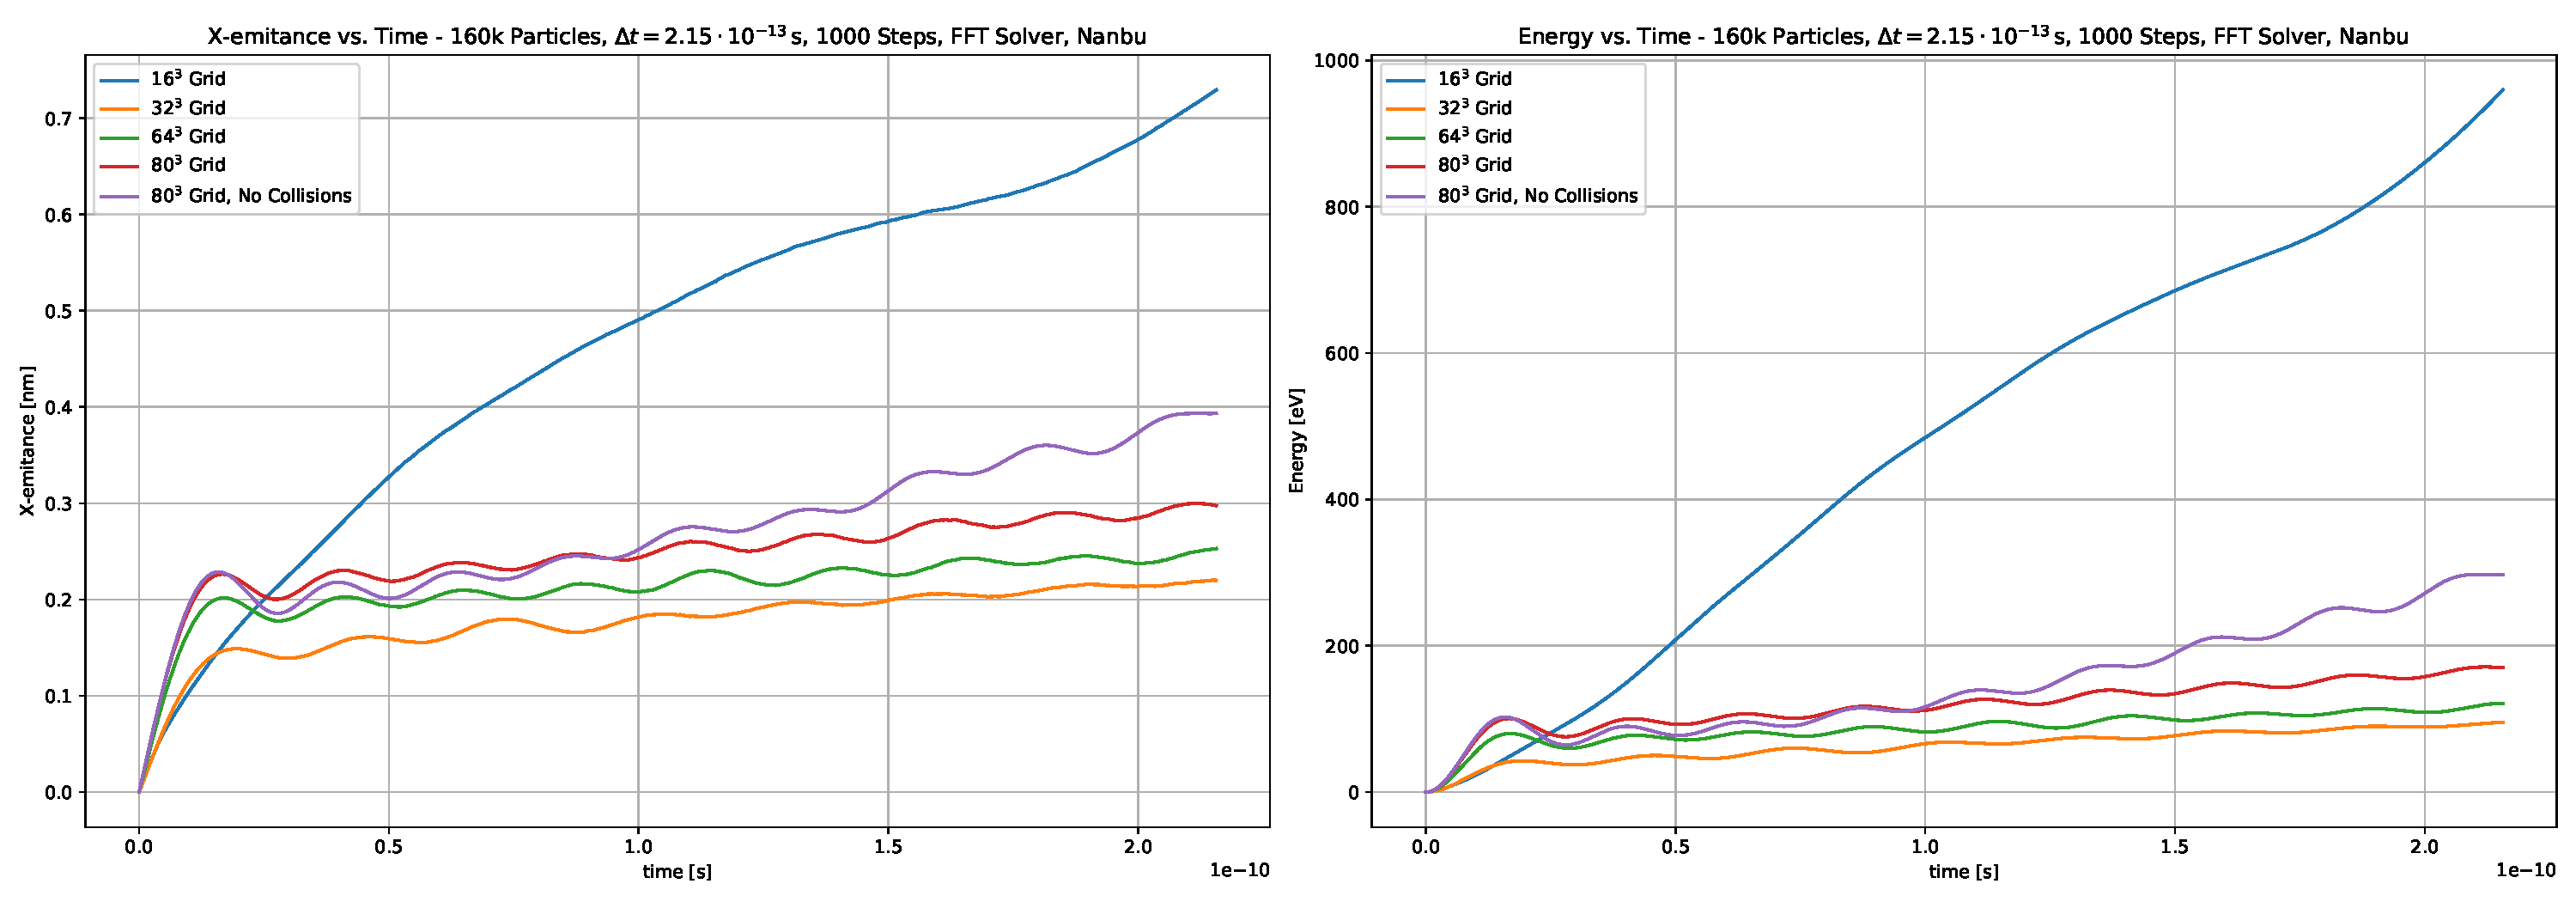
\includegraphics[width=\linewidth]{ressources/additional/disorder_heating_grid_comparison.pdf}
    \captionof{figure}{$x$-emittance and total energy against time for different mesh grid sizes.}\label{img:additional:disorder_heating_grid_comparison}
    \vspace{5pt}
\end{minipage}
The simulation was done using $156055$ particles and \textsc{Nanbu}'s collision algorithm.


\subsection{Scaling Issue in Adaptive Grid}

The analysis mentions a few issues with the scaling of the electrical field when using the adaptive grid for the field solver. 
\begin{description}
    \item[Problem description.] Consider the test case of a cold sphere. All particles are distributed in a $18\,\si{\micro\metre}$ sphere, while the simulation domain has $L = 100\,\si{\micro\metre}$. Therefore, we have a lot of free space around it. If we solve the field over the whole domain, we get a smaller field value than if we adapt the grid to exclude all the necessary free space. Even considering a similar ``grid density'' to match the number of particles per cell, with and without the adaptive grid, yields the same scaling issue. In this case, the field values lead to an $x$-emittance that is off by a factor of around $2.5$.
\end{description}
I did not find a solution to this problem yet. However, I detailed the exact steps the code takes to adapt the grid every timestep. Inside \verb|advance()|, calculate self-consistent field using:
\begin{lstlisting}
if (this->computeSelfField_m) {
    if (this->adjust_field_dims) adjustFieldMeshDimensions(); 
    this->par2grid();
    this->fsolver_m->runSolver();
    this->grid2par();
    if (this->adjust_field_dims) resetBoundaries();
}
\end{lstlisting}
Then adjust grid dimensions, such that every particle is barely in it. After solving and interpolating onto the particles, the boundaries are resetted to the value before (which are hardcoded at the moment according to the corresponding test case).

Now we can look at the actual grid adjustment:
\begin{lstlisting}
void adjustFieldMeshDimensions() {
    std::shared_ptr<ParticleContainer_t> pc = this->pcontainer_m;
    auto *mesh = &this->fcontainer_m->getMesh();
    auto *FL   = &this->fcontainer_m->getFL();

    // Calculate the maximum and minimum of all particle coordinates using Kokkos
    view_type* R               = &(pc->R.getView());
    MinMaxReducer<Dim> minMax;
    findMinMax(R, minMax); 
    Vector_t<double, Dim> maxR = minMax.max_val, minR = minMax.min_val;
    
    // Now figure out componentwise global min/max values
    Vector_t<double, Dim> globalMaxR, globalMinR;
    for (size_t i = 0; i < Dim; i++) {
        ippl::Comm->reduce(&maxR[i], &globalMaxR[i], 1, std::greater<double>());
        ippl::Comm->reduce(&minR[i], &globalMinR[i], 1, std::less<double>());
    }

    // Calculate new mesh spacing 
    Vector_t<double, Dim> hr = (globalMaxR-globalMinR) / mesh->getGridsize(); 
    
    // set the origin and mesh spacing of the mesh via
    mesh->setMeshSpacing(hr);
    mesh->setOrigin(globalMinR); 

    this->rmin_m = globalMinR;
    this->origin_m = globalMinR;
    this->rmax_m = globalMaxR;
    this->hr_m = hr;

    extLayoutUpdate(FL, mesh);
    pc->update();
}
\end{lstlisting}
Herem we manually reset \verb|rmin|, \verb|rmax|, recalculate \verb|hr| and update the mesh container.

The layout update is a bit more complicated and given in a new function:
\begin{lstlisting}
void extLayoutUpdate(ippl::FieldLayout<Dim>* fl, ippl::UniformCartesian<T, Dim>* mesh) {
    std::shared_ptr<ParticleContainer_t> pc = this->pcontainer_m;
    std::shared_ptr<FieldContainer_t> fc    = this->fcontainer_m;

    Field_t<Dim>* rho_m   = &(fc->getRho());
    VField_t<T, Dim>* E_m = &(fc->getE());

    rho_m->updateLayout(*fl);
    E_m->updateLayout(*fl);
    pc->getLayout().updateLayout(*fl, *mesh);
    
    std::get<FFTSolver_t<T, Dim>>(this->fsolver_m->getSolver()).setRhs(*rho_m);
}
\end{lstlisting}
This might include a few (technically) redundant updates. Additional \verb|updateLayout| calls did not make any differences. 

Finally, after the field is solved and interpolated onto the particle positions, the boundaries are resetted:
\begin{lstlisting}
void resetBoundaries() {
    this->origin_m = 0.0;
    this->rmin_m   = this->origin_m;
    if (this->initial_distr == "sphere") {
        this->rmax_m = 506.84;
    } else {
        this->rmax_m = 1.0;
    }
    this->hr_m     = this->rmax_m / this->nr_m;

    std::shared_ptr<ParticleContainer_t> pc = this->pcontainer_m;
    auto *FL = &this->fcontainer_m->getFL();
    auto *mesh = &this->fcontainer_m->getMesh();
    
    // set the origin and mesh spacing of the mesh via
    mesh->setMeshSpacing(this->hr_m);
    mesh->setOrigin(this->rmin_m); 
}
\end{lstlisting}
This manually resets \verb|rmin|, \verb|rmax| and recalculates \verb|hr|. Then, the mesh container is updated. We do not need to update \verb|rho_m|, since its layout is updated in the next call of \verb|adjustFieldMeshDimensions()|, which is before the next run of the solver.



